\chapter{Stochastic and dynamic routing}
Stochastic vehicle routing problems (SVRPs) were introduced in the late 60's by \citet{Tillman1969}. In a nutshell SVRPs consider than one or more problem parameters (e.g., demands, travel times) are unknown when the routes are planned. Despite being around for nearly 50 years, SVRPs have attracted much less attention than their deterministic counterparts. This is a somehow intriguing phenomenon considering that in practice most VRPs are stochastic by nature. This status quo is, however, slowly changing. With recent advances on big data and intelligent transportation systems, the industry is more demanding on routing technology that can exploit the knowledge encapsulated in the massively available amounts of data. The routing community has responded positively to this challenge. As \citet{Gendreau2016} point out, in the last 15 years the effort (and therefore the number of publications) devoted to SVRPs has substantially increased. This chapter summarizes our contributions to that effort. %These contributions are the result of the author's joint work with his Ph.D. advisers (A. Medaglia, Ch. Gu\'eret, B. Castanier, and N. Velasco), colleagues (J.G. Villegas, L.-M. Rousseau, and J.C. Goodson), and students (A. G\'omez, A. Sarmiento, R. Marino, and N. Kullman). We first discuss 

%The reader is referred to \citet{Gendreau2014,Gendreau2016} and \cite{Oyola2016,Oyola2016a} for recent and comprehensive surveys.

\section{Stochastic demands}

The vehicle routing problem with stochastic demands (VRPSD) is without any doubts the most studied variant of SVRP. In the VRPSD a set of geographically spread customers demand (or supply) a product that must be delivered (or collected) using a fleet of limited-capacity vehicles located at a central depot. The particular characteristic of the problem is that the exact quantities demanded (supplied) by each customer are only known upon the vehicle's arrival at the customer location (i.e., they are stochastic). It is assumed, however, that each customer's demand follows a known probability distribution. The main impact of stochastic demands is that they introduce uncertainty into the feasibility of the routes; depending on the demand realizations (i.e., the actual values), a vehicle may arrive at a customer without enough capacity to satisfy its demand.

To deal with uncertain demands in the VRPSD, researchers have explored models based on various solution frameworks including
chance-constraint programming, stochastic programming with recourse, dynamic programming, Markov decision models, and the multi-scenario approach. Each of these frameworks takes into accounts factors such as instance size, assumptions about available technology (e.g., real-time communication between vehicles and decision-makers), and assumptions about managerial policies (e.g., whether or not routes can be modified during their execution). For a complete discussion of the characteristics of each framework the reader is referred to \cite{Secomandi2009} and \cite{Pillac2013}.

The most widely studied models in the literature are those based on two-stage stochastic programming \citep{Cordeau2006}. As the name suggests, in this framework the problem is solved in two phases. In the first phase a set of \emph{a priori routes} is planned, and in the second phase the routes are executed. If there is a capacity constraint violation, or \emph{route failure}, a corrective action, known as \emph{recourse}, is taken to recover feasibility. In general, the recourse actions generate an extra cost known only after the second phase. Thus, the objective is to design during the first phase a set of routes that minimizes the sum of the cost of the a priori routes and the expected cost of the recourse actions.

The most traditional recourse action, known as \emph{detour-to-depot}, involves traveling back to the depot to restore the vehicle capacity, returning to the customer to complete the service, and then continuing the route as initially planned \citep{Savelsbergh1995}. However, more sophisticated approaches have been explored in the literature. These include performing preemptive trips to the depot in an attempt to avoid route failures \citep{Yang2000,Bianchi2004,Tatarakis2009,Pandelis2012}, assigning each vehicle a partner to provide back-up in the event of a failure \citep{Ak2007}, and assigning customers to two routes and move them from their primary to their backup route in case of a failure \citep{Erera2009}. Although the detour-to-depot has been criticized for its apparent ``lack of realism'', this policy provides a simple way to deal with route failures in practice. Moreover, \cite{Gendreau2016} also point out that the detour-to-depot policy produces routes that are \emph{tactically stable} (i.e., they do not vary much from their initial plan); a desirable characteristic from an operational perspective. From a more academic perspective, we would add that given the massive literature dealing with models built on top of it, the detour-to-depot policy provides a solid base to assess new algorithms for the VRPSD. All the contributions described in this subsection relay on models employing the detour-to-depot policy. 

Formally, the VRPSD can be defined on a complete and undirected graph $G=(\mathcal{V},\mathcal{E})$, where $\mathcal{V}=\{0,\ldots,n\}$ is the vertex set and $\mathcal{E}=\{(v,u):v,u \in \mathcal{V},v\neq u \}$ is the edge set. Vertices $v=1,\ldots, n$ represent the customers and vertex $v=0$ represents the depot. A weight $t_{e}$ is associated with edge $e=(v,u)=(u,v)\in \mathcal{E}$, and it represents the travel time between vertices $v$ and $u$. Each customer $v$ has a random demand $\tilde{\xi}_{v}$ for a given product. The customers are served using an unlimited fleet of homogeneous vehicles with capacity $Q$. In general, it is assumed that: i) each customer's demand follows an independent and known probability distribution, ii) the demand realizations $\vec{\xi}$ are nonnegative and less than the capacity of the vehicle, and iii) each customer's demand realization is not known until the vehicle arrives at the customer location.

A planned route $r$ is a sequence of vertices $r=(0,v_{1},\ldots,v_{i},\ldots,v_{n_r},0)$, where $v_i \in \mathcal{V}\setminus \{0\}$ and $n_r$ is the number of customers served by the route. Depending on the context, we may refer to route $r$ as an ordered set of edges
$r=\{(0,v_{1}),\dots,(v_{i-1},v_{i}),\dots,(v_{n_{r}},0)\}$. During the execution of a planned route, if a route failure occurs, that is, the capacity of the vehicle is exceeded, the detour-to-depot recourse is applied to recover the feasibility of the route. We denote by $Pr(v_i)$ the probability of a route failure occurring while serving customer $v_i\in r$. This \emph{failure probability} is given by

\begin{eqnarray}
\small
Pr(v_i)&=&\sum_{i=2}^{n_{r}}\sum_{f=1}^{i-1}Pr\left(\sum_{j=2}^{i-1}\tilde{\xi}_{v_{j}}\leq f\cdot Q < \sum_{j=2}^{i}\tilde{\xi}_{v_{j}}\right)
\label{eq.vrpsd.failure_prob}
\end{eqnarray}

\noindent where the probability term represents the probability of the $f^{th}$ failure occurring while serving customer $v_{i}$. For the details of the derivation of (\ref{eq.vrpsd.failure_prob}) see \citep{Teodorovic1992}. Note that the number and location of route failures are not known when the routes are planned. Therefore, although all travel times are (assumed to be) deterministic, the total duration of a route $\tilde{T}_r$ is a random variable which realization is only known when the route is completed. On the other hand, the probability distribution of $\tilde{T}_r$ may be computed when the route is planned (see $\S$ \ref{s.vrpsd-dc} for further details).

The VRPSD consists in determining a set $\mathcal{R}$ of planned routes that minimizes:

\begin{equation}
\small
E\left[C\right]=\sum_{r\in \mathcal{R}}E\left[l_r+G_r\left(\vec{\xi}\right)\right]=\sum_{r\in \mathcal{R}}l_{r}+\sum_{r\in\mathcal{R}}E\left[G_r\left(\vec{\xi}\right)\right]\label{eq.vrpsd.of}
\end{equation}

\noindent where $l_{r}$ denotes the planned length (planned cost) and $E\left[G_r\left(\vec{\xi}\right)\right]$ the expected length of the returning trips to the depot, or cost of recourse, caused by route failures for each route $r\in \mathcal{R}$. The planned cost of a route is given by the sum of the lengths of the arcs traversed by the route. On the other hand, the estimation of the expected cost of recourse is slightly more complicated. Under the detour-to-depot recourse action, the expected cost of the failures in a route is given by:

\begin{eqnarray}
\small
E\left[G_r\left(\vec{\xi}\right)\right]&=&2\times \sum_{i=2}^{n_{r}}\sum_{l=1}^{i-1}Pr\left(\sum_{j=2}^{i-1}\xi_{v_{j}}\leq l\cdot Q < \sum_{j=2}^{i}\xi_{v_{j}}\right)\times d_{v_{i},0}
\label{eq.vrpsd.recourse}
\end{eqnarray}

The expected cost of failures in (\ref{eq.vrpsd.recourse}) can be efficiently computed when customer demands follow a probability function with the cumulative property. This property states that the sum of two independent and $\Psi$ distributed random variables is also $\Psi$ distributed, as it is the case for the normal, Poisson, and Gamma distributions.

\subsection{Solving the VRPSD}\label{s.vrpsd.msh}
The literature reports on several exact and heuristic approaches to tackle the VRPSD. Exact methods include that of \cite{Laporte2002a} who proposed an implementation of the L-Shaped algorithm and solved to optimality instances of up to 50 and 100 customers of a variant with limited fleet. In the same vein, \cite{Rei2007} proposed an implementation of the L-Shaped algorithm with local branching cuts for a variant in which a single route servicing all customers is to be designed (this problem is usually referred in the literature as the SVRPSD). The authors reported optimal solutions for instances of up to 90 customers with uniformly distributed demands. \cite{Christiansen2007} proposed a branch-and-price algorithm to tackle the baseline formulation. Their approach successfully solved instances of up to 60 customers with Poisson distributed demands. That algorithm was recently re-implemented and improved by \cite{Gauvin2014} who currently hold the best exact results for the problem. In the segment of heuristic approaches, \citet{Gendreau1996a} proposed a tabu search (TS) algorithm, known as \emph{tabustoch}, designed to tackle an extension of the baseline formulation in which, in addition to the demands, customers are also stochastic (i.e., they are present, or not, with a given probability). \citet{Yang2000} introduced two constructive heuristics for another extended formulation in which preventive trips to the depot are allowed. A similar formulation was proposed by \citet{Bianchi2006a} in the context of the SVRPSD. To solve their problem, these authors introduced a set of metaheuristics comprising simulated annealing (SA), iterated local search, ant colony optimization, evolutionary algorithms, and TS. More recently, \citet{Rei2010} introduced a hybrid Monte Carlo local branching approach for the SVRPSD. \citet{Goodson2012} introduced a hybrid simulated annealing that embeds sophisticated neighborhood schemes into a local search procedure. To our knowledge the most recent metaheuristic for the VRPSD is the variable neighborhood search algorithm of \cite{Sarasola2016}.

In joint work with Juan G. Villegas (UdeA, Colombia) we proposed the multi-space sampling heuristic (MSH) to solve the VRPSD. MSH works in two phases. In the first phase (sampling phase), it uses a set $H$ of \emph{sampling heuristics} to draw $T$ elements from the set of TSP-like tours (i.e., $\mathcal{P}$) and maps each sampled element $p^{t}$ to a sub-set $\Omega^t$ in the set of feasible routes (i.e., $\mathcal{T}$). In the second phase (mapping phase), the approach maps a set $\Omega\subset\mathcal{T}$, where $\Omega=\Omega^1\cup \ldots \cup \Omega^T$, to one element $s\in\mathcal{S}$ by solving a set-partitioning formulation of the problem. Algorithm \ref{AlgGeneralStructure} presents the general structure of the proposed heuristic.

\begin{algorithm}
\scriptsize
\caption{Multi-space sampling heuristic: general structure}\label{AlgGeneralStructure}
\begin{algorithmic}[1]
\Function{MultiSpaceSampling}{$G$,$H$}
    \State $t\leftarrow1$
    \State $\Omega\leftarrow\emptyset$
    \While{$t\leq T$}\label{samplingStart}
        \For{$k=1$ \textbf{to} $k=|H|$}
            \State $h\leftarrow H_{k}$
            \State $p^{t}\leftarrow h(G)$ \label{drawSample}
            \State $\langle\Omega^{t},s^{t}\rangle\leftarrow$\emph{s-split}$(G,p^{t})$ \label{split}
            \State $\Omega\leftarrow \Omega \cup \Omega^{t}$\label{updateOmega}
            \If{$t=1$} \label{saveBestStart}
                \State $s^*\leftarrow s^{t}$
            \ElsIf{$f(s^{t})< f(s^*)$}
                \State $s^*\leftarrow s^{t}$
            \EndIf \label{saveBestEnd}
            \State $t\leftarrow t+1$
        \EndFor
    \EndWhile\label{samplingEnd}
    \State $s^*\leftarrow setPartitioningProblem(G,\Omega,s^*)$\label{mapping}
    \State \Return $\mathcal{R}\leftarrow s^*$
\EndFunction
\end{algorithmic}
\end{algorithm}

To draw elements from $\mathcal{P}$ (line \ref{drawSample} in Algorithm \ref{AlgGeneralStructure}), we use randomized versions of 4 different TSP constructive heuristics: randomized nearest neighbor (RNN), randomized nearest insertion (RNI), randomized best insertion (RBI), and randomized farthest insertion (RFI). Although the strategies used to generate the randomized versions of the four heuristics are rather intuitive, for the sake of completeness we briefly describe them here.

Let $p$ be the TSP tour being built by a given sampling heuristic, $\mathcal{W}$ the set of vertices visited by $p$, and $\mathcal{N}=\mathcal{V}\setminus \mathcal{W}$ an ordered set of not-routed vertices. For the sake of simplicity, we assume that sets $\mathcal{W}$ and $\mathcal{N}$ are updated every time a customer is added to $p$. Let us also define three metrics for every customer $v\in\mathcal{N}$, namely, $d_{min}(v)=\min\{d_{v,u}|u\in \mathcal{W}\}$, $d_{max}(v)=\max\{d_{v,u}|u\in \mathcal{W}\}$, and $\Delta_{min}(v)=\min\{d_{u,v}+d_{v,w}-d_{u,w}|(u,w)\in p\}$. Finally, let $k$ be a random integer selected in $[1,\min\{K,|\mathcal{N}|\}]$, where parameter $K$ denotes the \emph{randomization factor} of each heuristic. The four sampling heuristics operate as follows:

\begin{itemize}
\small
\item \textbf{RNN:} Set $p=\{0\}$ and $u=0$. At each iteration: identify the vertex $v$ who is the $k_{th}$ nearest vertex to $u$, append $v$ to $p$, and set $u=v$. Stop when $|\mathcal{N}|=0$ and append $0$ to $p$ to complete a tour.
\item \textbf{RNI:} Initialize $p$ as a tour starting at the depot and performing a round trip to a randomly selected customer (henceforth this procedure will be referred simply as initialize $p$). At each iteration: sort $\mathcal{N}$ in non-decreasing order of $d_{min}(v)$. Insert $v=\mathcal{N}_{k}$ in the best possible position in the tour (i.e., the position generating the shortest increment in the cost of the tour). Stop when $|\mathcal{N}|=0$.
\item \textbf{RFI:} Initialize $p$. At each iteration: sort $\mathcal{N}$ in non-decreasing order of $d_{max}(v)$ and insert $v=\mathcal{N}_{k}$ in the best possible position in the tour. Stop when $|\mathcal{N}|=0$.
\item \textbf{RBI:} Initialize $p$. At each iteration: sort $\mathcal{N}$ in non-decreasing order of $\Delta_{min}(v)$ and insert $v=\mathcal{N}_{k}$ in the best possible position in the tour. Stop when $|\mathcal{N}|=0$.

\end{itemize}

To map each sampled element $p^{t}$ to its corresponding $\Omega^p\subset\mathcal{T}$ (line \ref{split} in Algorithm \ref{AlgGeneralStructure}) our approach uses the s-split procedure for the VRPSD \cite{Mendoza2010}. S-split was originally proposed to map an element in $\mathcal{P}$ to an element in $\mathcal{S}$ by optimally partitioning the giant tour into a set of feasible routes that form a VRPSD solution. Nonetheless, s-split  accomplishes its mission by running a dynamic programming algorithm that evaluates every single feasible route that can be obtained from the giant tour without altering the order of the customers. In other words, by saving a reference to the set of routes evaluated by s-split while partitioning $p^{t}$, we obtain a mapping of $p^{t}$ to a sub-set $\Omega^{t}\subset\mathcal{T}$. Since s-split also retrieves a mapping of $p^{t}$ to a solution $s^{t}\in\mathcal{S}$, we keep a reference to the best solution found during the sampling phase (lines \ref{saveBestStart}--\ref{saveBestEnd} in Algorithm \ref{AlgGeneralStructure}) to have a good upper bound in the second phase of our heuristic. The leftmost frame in Figure \ref{FigExample} illustrates the operation of s-split in an execution of the proposed heuristic with $H=\{RFI,RNI\}$ and $T=2$. For all details needed to implement s-split the reader is referred to \cite{Mendoza2010,Mendoza2011}.

In the second phase, our approach maps the set $\Omega=\Omega^1\cup \ldots \cup \Omega^T$ to a solution $s^{*}\in\mathcal{S}$ by solving a set-partitioning formulation of the VRPSD proposed by \citet{Christiansen2007} $\left( \min_{\mathcal{R}\subseteq \Omega} \left\{ \sum_{r\in \mathcal{R}}E[C_{r}]: \bigcup_{r \in \mathcal{R}}=\mathcal{V} ;  r_i \bigcap r_j=\{0\} \, \forall r_i,r_j \in  \mathcal{R} \right\}\right)$. The objective is then to select the best sub-set of routes from $\Omega$ to build the set of planed routes $\mathcal{R}$ (i.e., solution) ensuring that each customer will be visited by exactly one route. The rightmost frames in Figure \ref{FigExample} illustrate the operation of the mapping phase in our heuristic.

In most VRP variants, it is possible to replace the set-partitioning formulation of the problem by an equivalent set-covering formulation aiming to gain in computational efficiency. This approach is based in the premise that the cheapest way to cover all customers is to cover them only once because the cost verifies the triangle inequality. Therefore, the optimal solution of the set-covering problem is a feasible VRP solution. In the VRPSD, however, that is not necessarily the case. Indeed, because the expected cost of failing while visiting a customer $v$ depends on the expected demands of all customers previously visited by the route and on its distance to the depot, see Equation (\ref{EqRecourse}), there is no guarantee that a route $r=(0,\ldots,u,v,\ldots,0)$ has a total expected cost $E[C_{r}]$ that is cheaper than that of a route $r'=(0,\ldots,u,w,v,\ldots,0)$. Hence, the cheapest way to cover all customers may include covering some customers more than once, which leads to an unfeasible VRPSD solution. One can overcome this difficulty by implementing an ad-hoc verification and reparation procedure. After some preliminary experimentation using a set-covering formulation in the mapping phase, we assessed that the benefits obtained in terms of computational efficiency did not pay off the loss in simplicity of our heuristic, so we kept the original set-partitioning formulation.

It is worth mentioning that although in many VRP variants excellent solutions can be found by solving set-covering/set-partitioning formulations over a reduced set of routes, researchers often oversight the benefits of embedding this kind of component in heuristic procedures. Authors like Villegas et al. \cite{Villegas2011}, however, have shown that applied as a post-optimization procedure, this approach may lead to significant improvements in the quality of final solutions. We consider important to remark that in the proposed heuristic, the set-partitioning model is an integral part of the method rather than only a post-optimization strategy.


\begin{figure}
\begin{center}
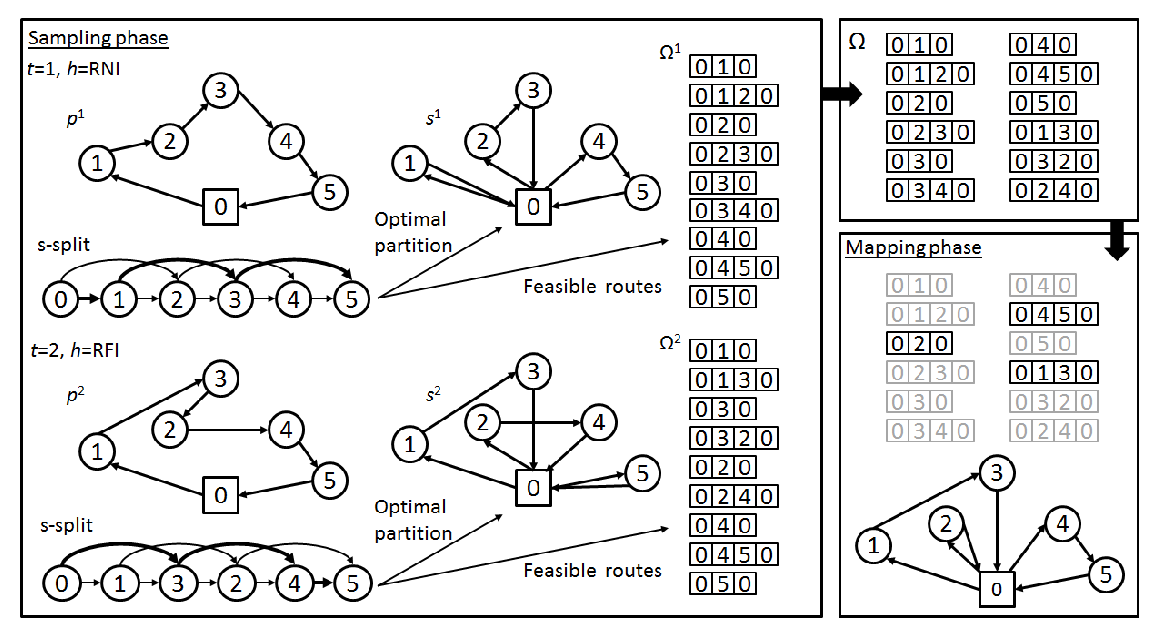
\includegraphics[width=12cm,clip=true]{./img/msh_example}
\caption{Multi-space sampling heuristic: example of an execution with $H=\{RNI,RFI\}$ and $T=2$}\label{FigExample}
\end{center}
\end{figure}

\subsection{Handling duration constraints}\label{s.vrpsd-dc}
One of the most challenging issues when solving the VRPSD and its variants is dealing with duration constraints (DCs). It is easy to see that recourse actions add travel time to the planned routes. Since the exact number of recourses and the extra time they add to each route is not known when the routes are planned, the total duration of a route is itself a random variable. The latter may lead to a problem in practice if the routes are subject to DCs.

Duration constraints have been studied only rarely in the context of the VRPSD. To the best of our knowledge, the body of work in this domain is limited to about ten references, most of them focusing on approaches based on two-stage stochastic programming. For the sake of brevity, in the remainder of this subsection we focus on these approaches; however, we refer the reader to the excellent papers by \citet{Bent2004,Bent2007} and \citet{Goodson2013,Goodson2013a} for research based on other frameworks.

\citet{Yang2000} is probably the first reference to DCs in the VRPSD literature. The authors handle these constraints by imposing a limit on the expected duration of the a priori routes. \citet{Mendoza2010,Mendoza2011} applied the same strategy in the context of the multi-compartment VRPSD (MC-VRPSD), a problem in which each customer demands several incompatible products that are transported in different vehicle compartments. The main advantage of this \emph{constrained expected duration} approach is its computational convenience. Indeed, since the expected duration of a route is usually computed as part of the objective function, the DC feasibility check requires no additional effort. On the other hand, although this strategy may be adequate for practical situations where DCs are rather soft constraints, it does not provide decision-makers with an explicit mechanism to express their preferences about violations of these constraints.

\citet{Tan2007} and \cite{Sorensen2009} propose an alternative approach, based on penalizing violations of the DCs in the objective function. \citet{Tan2007} use the penalties as part of a cost function called drivers' remuneration that they optimize, along with the total traveled distance and the number of vehicles, using a multi-objective optimization approach. \cite{Sorensen2009} include the penalties directly in the total-duration objective function and use an established mono-objective approach \citep{Sorensen2006a} to solve the problem. In both cases, the authors use Monte Carlo simulation to generate multiple scenarios of the demand realizations that are used to compute the total expected duration of the routes and the penalties for DC violations. \cite{Mendoza2009b} propose a different strategy to address DCs in the context of a bi-objective MC-VRPSD: they minimize simultaneously the total expected cost of a set of routes and its coefficient of variation. In their approach, DCs are imposed on planned routes as \emph{chance constraints} ensuring that the probability of completing a route in less than its maximum duration is greater than a given threshold. To perform the feasibility check of the chance constraints, the authors use Monte Carlo simulation.

From the conceptual point of view, both the penalty and chance-constraint approaches overcome the shortcomings of the constrained expected-duration approach. However, the implementations based on Monte Carlo simulation may be unnecessarily expensive from a computational point of view because one may need to generate a large number of scenarios to achieve statistical significance. \citet{Haugland2007} and \citet{Erera2010} propose approaches for applications in which the DCs are hard constraints. In \cite{Haugland2007} the authors solve a VRPSD with DCs as part of the evaluation of the solution to a districting problem. To check the DC feasibility the authors use an upper bound on the total duration of a route. \citet{Erera2010} propose an algorithm to compute the maximum duration of a route for any realization of the customer demands. They use its result as an input to check the DCs.

In joint work with J.G. Villegas (UdeA, Colombia) and L.-M. Rousseau (CIRRELT, Canada), carried between 2012 and 2013, we revisited the penalty and chance-constraint strategies to deal with DCs in the VRPSD. One of the most important contributions of our work is that in contrast to previous approaches, we did not use Monte Carlo simulation to evaluate routes. We instead devised a mechanism for explicitly building the probability distribution of the duration of a route. In the remainder of this subsection we briefly discuss this and other contributions to the VRPSD with DCs (VRPSD-DC); full details can be found in \citep{Mendoza2015}.

\subsubsection{Computing the probability distribution of the duration of a route}
Note that according to the VRPSD definition given in \ref{s.vrpsd.definition} all the demand realizations are less than the capacity of the vehicle. Therefore, a route may fail at the most once at each customer but the first one. In other words, the maximum number of failures in a route is $n_{r}-1$, and the first failure cannot occur while serving the first customer. Consequently, $\tilde{T}_{r}$ follows a discrete distribution with $2^{n_r-1}$ possible outcomes; we refer to each of these outcomes as a \emph{duration profile}. Figure \ref{f.vrpsd.dc.profiles} illustrates this concept. Let $\mathcal{P}(r)$ be the set of all possible duration profiles for route $r$. Let $Pr(p)$ be the probability of observing duration profile $p\in\mathcal{P}(r)$, and let $T_{r}(p)$ be the total duration of route $r$ if profile $p$ is observed. The leftmost part of the figure depicts a planned route $r=\{(0,a),(a,b),(b,c),(c,0)\}$ with a total planned duration $t_{r}=\sum_{(u,v)\in r}t_{(u,v)}=t_{(0,a)}+t_{(a,b)}+t_{(b,c)}+t_{(c,0)}$. The rightmost part of the figure shows a tree in which each leaf node represents one possible duration profile $p$ for route $r$. For instance, leaf node $p=1$ represents the duration profile of the route if failures occur while serving customers \emph{b} and \emph{c}. In such case, $T_r(p)=t_r+2t_{(b,0)}+2t_{(c,0)}$ and $Pr(p)=\left(1-Pr(a)\right)\times Pr(b) \times Pr(c)$, where $Pr(a)$, $Pr(b)$, and $Pr(c)$ denote the probability of having a failure while servicing customers \emph{a}, \emph{b}, and \emph{c}, respectively (see Equation (\ref{eq.vrpsd.failure_prob})). It is worth mentioning that since failures cannot occur while servicing customer \emph{a}, the upper branches of the three (in grey) represent impossible duration outcomes. Building on top of our duration profiles we proposed two stochastic programming formulation for the VRPSD-DC.

\begin{figure}
    \begin{center}
    \includegraphics[width=9cm,clip=true]{./img/fvrpsddcprofiles}
    \caption{Duration profiles for a given route and their attributes}\label{f.vrpsd.dc.profiles}
    \end{center}
\end{figure}

\subsubsection{Chance-constraint formulation}\label{s.vrpsd.dc.CC}
In our first formulation we extend the classical two-stage stochastic programming formulation for the VRPSD to include the DCs as chance constraints. The resulting problem involves finding a set $\mathcal{R}$ of planned routes that minimizes

\begin{eqnarray}\label{eq.vrpsd.dc.CC}
\small
E\left[C_1(\mathcal{R})\right] &=&\sum_{r\in\mathcal{R}}E\left[\tilde{T}_r\right]\label{eq.vrpsd.dc.CC.OF}
\end{eqnarray}
\noindent s.t.
\begin{eqnarray}
\small
\label{eq.vrpsd.dc.CC.DC} \sum_{r\in\mathcal{R}}Pr\left(\tilde{T}_r>T\right)&\leq&\beta\ \ \ \ \ \ \ \ \forall \ r\in \mathcal{R}\\
\label{eq.vrpsd.dc.CC.QC} \sum_{i\in r}E\left[\tilde{\xi}_{v_i}\right]&\leq&Q\ \ \ \ \ \ \ \ \forall \ r\in \mathcal{R}\\
\label{eq.vrpsd.dc.CUSTOMER-COVERTURE} r\bigcap r'&=&\{0\}\ \ \ \ \ \ \forall \ r,r'\in\mathcal{R},r\neq r'\\
\label{eq.vrpsd.dc.SINGLE-VISIT} \bigcup_{r\in \mathcal{R}}&=&\mathcal{V}
\end{eqnarray}

The objective (\ref{eq.vrpsd.dc.CC.OF}) minimizes the total expected duration of the set of routes $\mathcal{R}$. Constraint (\ref{eq.vrpsd.dc.CC.DC}) ensures that the probability that a route violates the duration limit is lower than a given threshold $\beta$. Using the duration profiles of route $r$ as an input, the first term in (\ref{eq.vrpsd.dc.CC.DC}) can be computed as

\begin{eqnarray}\label{eq.vrpsd.dc.CC.pr}
\small
\label{eq.vrpsd.dc.CC.DC-COMPUTATION} Pr\left(\tilde{T}_r> T\right)&=&\sum_{p\in \mathcal{P}(r)|T_{r}(p)>T}Pr(p).
\end{eqnarray}

\noindent Constraint (\ref{eq.vrpsd.dc.CC.QC}) ensures that each planned route is designed so that the total expected load does not exceed the capacity of the vehicle while constraints (\ref{eq.vrpsd.dc.CUSTOMER-COVERTURE}) and (\ref{eq.vrpsd.dc.SINGLE-VISIT}) guarantee that each customer is included in one and only one planned route.

\subsubsection{Penalty formulation}\label{s.vrpsd.dc.P}

In our second formulation we follow a completely different approach. To account for the DCs, we extend the classical VRPSD objective to include the expected cost of overtime, i.e., the time that each route travels above the limit $T$. In this formulation the problem involves finding a set of planned routes $\mathcal{R}$ verifying constraints (\ref{eq.vrpsd.dc.CC.QC})--(\ref{eq.vrpsd.dc.SINGLE-VISIT}) and minimizing

\begin{eqnarray}\label{eq.vrpsd.dc.P}
\small
\label{eq.vrpsd.dc.P.OF} E\left[C_2(\mathcal{R})\right] &=&\sum_{r\in\mathcal{R}}E\left[\tilde{T}_r\right] + E\left[\phi\left(\tilde{O}_r\right)\right]
\end{eqnarray}
\noindent where
\begin{eqnarray}
\small
\label{eq.vrpsd.dc.phi}
E\left[\phi\left(\tilde{O}_r\right)\right] & = & \sum_{p\in \mathcal{P}(r)|T_{r}(p)>T}\phi\left(T_{r}(p)-T\right)\times Pr(p)
\end{eqnarray}

\noindent is the expected overtime cost. Function $\phi(\cdot)$ models the decision maker's aversion toward overtime. It can take any form depending on the context. For instance, quadratic functions can model situations in which even small violations of the DCs should be discouraged, while piecewise linear functions can be useful when small violations are acceptable but violations beyond a given threshold should be avoided.

In the remainder of the subsection, we refer to our chance-constraint and penalty formulations as \verb"CC" and \verb"PF".

\subsubsection{A hybrid metaheuristic}\label{s.vrpsd.dc.grasp}
To solve our two formulations for the VRPSD-DC, namely \texttt{CC} and \texttt{PF}, we developed a GRASP with HC. Algorithm \ref{a.vrpsd.dc.grasp} describes the proposed approach. At the $k$th GRASP iteration  (lines \ref{a.vrpsd.dc.grasp.start}--\ref{a.vrpsd.dc.grasp.end}) we greedily construct a starting solution (lines \ref{a.vrpsd.dc.grasp.randTSP}--\ref{a.vrpsd.dc.grasp.split}) and then try to improve it using a local search procedure (line \ref{a.vrpsd.dc.grasp.vnd}). To construct the starting solution, we select a randomized TSP heuristic $h$ from a predefined set $\mathcal{H}$ and use it to build a giant TSP tour $tsp^{k}$ visiting all the customers (line \ref{a.vrpsd.dc.grasp.randTSP}). We then use an adaptation of the s-split procedure for the VRPSD \citep{Mendoza2011} to optimally partition $tsp^{k}$ into a set of feasible routes that forms a starting solution $s^{k}$ (line \ref{a.vrpsd.dc.grasp.split}). We next launch a VND procedure from the starting solution $s^{k}$ (line \ref{a.vrpsd.dc.grasp.vnd}). At the end of iteration $k$, we update the best solution $s^{*}$ (line \ref{a.vrpsd.dc.grasp.updateBest}) and add the routes of the local optimum (i.e., $s^k$) to a set $\Omega$ (lines \ref{a.vrpsd.dc.grasp.updateOmega.start}--\ref{a.vrpsd.dc.grasp.updateOmega.end}). After $K$ iterations the GRASP stops and we carry out the HC. In this phase, our method solves a set partitioning problem (SPP) over the set of routes $\Omega$ (line \ref{a.vrpsd.dc.grasp.hc}). Note that the specific implementations of \verb"split"($\cdot$) and \verb"vnd"($\cdot$) vary depending on the formulation (i.e., \texttt{CC} or \texttt{PF}) being solved, whereas the implementations of \verb"tsp"($\cdot$), \verb"update"($\cdot$), and \verb"setPartitioning"($\cdot$) are unchanged. For a thorough description of the algorithmic components embedded into our GRASP as well as a full description of how the split procedure was adapted to work on \texttt{CC} and \texttt{PF} the reader is referred to \cite{Mendoza2015}.

\begin{algorithm}[h]
\small
\caption{GRASP+HC: General structure}
\label{a.vrpsd.dc.grasp}
\begin{algorithmic}[1]
\Function{GRASPHC}{$\mathcal{H}$,$K$,\texttt{mode}} \Comment \textsf{mode}=$\{\texttt{CC},\texttt{PF}\}$
    \State $\Omega\leftarrow\emptyset$, $k\leftarrow1$
    \While{$k\leq K$} \label{a.vrpsd.dc.grasp.start}
        \For{$h \in \mathcal{H}$}
            \State $tps^{k}\leftarrow$\verb"tsp"$(h)$ \label{a.vrpsd.dc.grasp.randTSP}
            \State $s^{k}\leftarrow$\verb"split"$(tsp^{k},\textsf{mode})$\label{a.vrpsd.dc.grasp.split}
            \State $s^{k}\leftarrow$\verb"vnd"$(s^{k},\textsf{mode})$\label{a.vrpsd.dc.grasp.vnd}
            \State $s^*\leftarrow$\verb"update"$(s^{k},s^*)$\label{a.vrpsd.dc.grasp.updateBest}
            \For{$r\in s^{k}$}\label{a.vrpsd.dc.grasp.updateOmega.start}
                \State $\Omega\leftarrow \Omega \cup r$
            \EndFor\label{a.vrpsd.dc.grasp.updateOmega.end}
            \State $k\leftarrow k+1$
        \EndFor
    \EndWhile\label{a.vrpsd.dc.grasp.end}
    \State $\mathcal{R}\leftarrow$ \verb"setPartitioning"$(\Omega,s^*)$\label{a.vrpsd.dc.grasp.hc}
    \State \Return $\mathcal{R}$ \label{a.vrpsd.dc.grasp.return}
\EndFunction
\end{algorithmic}
\end{algorithm}

\subsubsection{Some results}

\noindent \textit{Classical VRPSD}\\
It is worth nothing that solving the classical VRPSD is equivalent to solving \texttt{CC} with $\beta=1$ (i.e., the DC becomes redundant). For validation purposes, we tested our approach on the classical VRPSD. We ran our hybrid metaheuristic on the 40-instance testbed of \citet{Christiansen2007}. These instances range from 16 to 60 customers and assume Poisson-distributed demands. To assess the effectiveness of our method, we compared our results to the best known solutions (BKSs) for the testbed: 38 optimal solutions reported by \cite{Gauvin2012} and 2 heuristic solutions reported by \cite{Goodson2012} and \cite{Mendoza2013}.

The results showed that in terms of solution quality our approach outperforms the two state-of-the-art metaheuristics: it matched the 40 BKSs for the set, whereas \cite{Mendoza2013} achieved 27/40 and \cite{Goodson2012} achieved 33/40. Although it was difficult to make a precise comparison of the computational performance because of slight differences in the testing environments, the results also suggested that our approach outperforms the two other methods on this measure. To the best of our knowledge, our approach is still the state-of-the-art metaheuristic to tackle the VRPSD, despite the more recent publication of the \citeauthor{Sarasola2016} variable neighborhood search.

\subsection{The case of multi-compartment vehicles}
	Papers: Mendoza et al. (2010,2011)
\subsection{The trade-off between expected cost and variance}
	Conference paper: Mendoza et al. (2009)
\section{Stochastic travel and service times}
  	Paper: Gómez et al. (2016)
\subsection{Handling correlated parameters}
  	Working paper: Sarmiento et al. (2016)
\section{Perspectives}
  	\subsection{Combining optimization and machine learning}
  	On going Ph.D. Thesis: Mustapha Haouassi
